\documentclass{article}
\usepackage{tikz}
\usetikzlibrary{positioning}
\usepackage[margin=0.5in]{geometry}
\pagestyle{empty}
\begin{document}
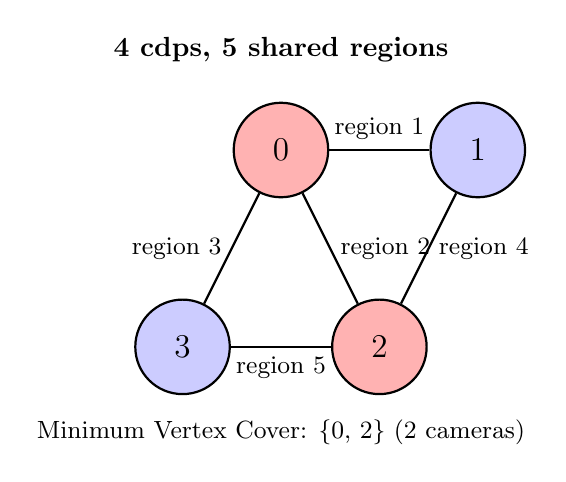
\begin{tikzpicture}[
  node distance=2.5cm,
  cdp/.style={circle, draw, fill=blue!20, minimum size=1.2cm, font=\large, thick},
  selected/.style={circle, draw, fill=red!30, minimum size=1.2cm, font=\large, thick},
  edge/.style={thick, black}
]
  % Vertices (cdps) - arranged in a square with vertex 0 at top
  \node[selected] (0) at (0,2.5) {0};  % Selected in minimum cover
  \node[cdp] (1) at (2.5,2.5) {1};
  \node[selected] (2) at (1.25,0) {2};  % Selected in minimum cover
  \node[cdp] (3) at (-1.25,0) {3};
  
  % Edges (shared regions) - 5 edges total
  \draw[edge] (0) -- node[above, sloped, font=\small] {region 1} (1);
  \draw[edge] (0) -- node[right, font=\small] {region 2} (2);
  \draw[edge] (0) -- node[left, font=\small] {region 3} (3);
  \draw[edge] (1) -- node[right, font=\small] {region 4} (2);
  \draw[edge] (2) -- node[below, font=\small] {region 5} (3);
  
  % Title
  \node[above] at (0,3.5) {\textbf{4 cdps, 5 shared regions}};
  \node[below] at (0,-0.8) {\small Minimum Vertex Cover: \{0, 2\} (2 cameras)};
\end{tikzpicture}
\end{document}

